\subsection{Teilaufgabe 2}
\subsubsection{Aufgabenstellung}
In der Zweiten Teilaufgabe sollen wir uns mit den Wertebereichen der Primitiven Datentypen befassen und
deren Wertebereiche in einem Programm ausgeben.

\subsubsection{Anforderungsdefinition}
\begin{enumerate}
	\item Zu jedem primitiven Datentypen den Max und Min-Wert ausgeben.
\end{enumerate}

\subsubsection{Entwurf}
\begin{center}
	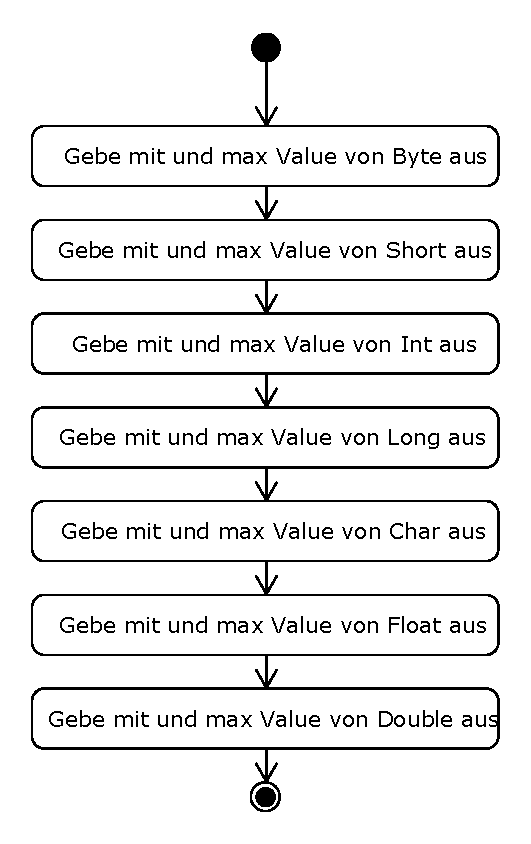
\includegraphics[width=0.5\textwidth]{uml/uml_c3_p2.pdf}
\end{center}

\subsubsection{Quelltext}
\paragraph{Wertebereiche.java}\
\lstinputlisting[language = Java , frame = trBL , escapeinside={(*@}{@*)}]{../chapter_03/src/main/java/chapter_03/Wertebereiche.java}


\subsubsection{Testdokumentation}
Nach dem Start des Programms sollten die Min und Max werte der einzelnen Datentypen ausgegeben
werden. Anschlie\ss end wurden die Werten mit den in der Java Dokumentation stehenden Werten
verglichen. Alles hat soweit gestimmt.

\subsubsection{Benutzungshinweise}
Keine Besonderen Benutzungshinweise.
Man navigiere zu dem Ordner von sich die Compilierte Datei mit dem Namen "Wertebereiche.class"
\space befindet und führt anschlie\ss end java Wertebereiche aus.

\subsubsection{Anwendungsbeispiel}
Nach dem man das Programm gestartet hat (aufgrund der Formatierung, werden einige Zeichen bei Char nicht dargestellt), sollte folgende Ausgabe erscheinen:

\begin{lstlisting}[frame = trBL , firstnumber = last , escapeinside={(*@}{@*)}]
[sebastian@laptop bin]$ java Wertebereiche
Byte min -128 | Byte max 127
Short min -32768 | Short max 32767
Integer min -2147483648 | Integer max 2147483647
Long min -9223372036854775808 | Byte Long 9223372036854775807
Char min  | Char max ￿
Float min 1.4E-45 | Float max 3.4028235E38
Double min 4.9E-324 | Double max 1.7976931348623157E308
[sebastian@laptop bin]$ 
\end{lstlisting}